%\documentclass[journal]{IEEEtran}
\documentclass[12pt, draftcls, onecolumn]{IEEEtran}
\makeatletter
% journal (default) and conference
\def\subsubsection{\@startsection{subsubsection}% name
                                 {3}% level
                                 {\z@}% indent (formerly \parindent)
                                 {0ex plus 0.1ex minus 0.1ex}% before skip
                                 {0ex}% after skip
                                 {\normalfont\normalsize\bfseries}}% style
\makeatother
\usepackage[T1]{fontenc}% optional T1 font encoding
%\usepackage{graphicx}
\usepackage{subfigure}
\usepackage{ulem}
\usepackage{amsmath}
\allowdisplaybreaks
\usepackage{hhline}
\usepackage{yfonts,color}
\usepackage{soul,xcolor}
\usepackage{verbatim}
\usepackage{amsmath}
\allowdisplaybreaks
\usepackage{amssymb}
\usepackage{amsthm}
\usepackage{float}
\usepackage{bm}
\usepackage{url}
\usepackage{array}
\usepackage{cite}
\usepackage{graphicx}
\usepackage{framed} % for frame
\usepackage{balance} % balance
\usepackage{epsfig,epstopdf}
\usepackage{booktabs}
\usepackage{courier}
\usepackage{subfigure}
\usepackage{pseudocode}
\usepackage{enumerate}
\usepackage{algorithm}
\usepackage{algpseudocode}
\usepackage[export]{adjustbox}
\newtheorem{definition}{Definition}
\newtheorem{theorem}{Theorem}
\newtheorem{lemma}[theorem]{Lemma}
\newtheorem{proposition}[theorem]{Proposition}
%\newtheorem{proposition}{Proposition}
\newtheorem{corollary}[theorem]{Corollary}
\newtheorem{assumption}{Assumption}
\newtheorem{remark}{Remark}
\renewcommand{\algorithmicrequire}{\textbf{Initialization:}}  % Use Input in the format of Algorithm
\renewcommand{\algorithmicensure}{\textbf{Output:}}  % Use Output in the format of 
\newcommand{\rom}[1]{\uppercase\expandafter{\romannumeral #1\relax}}
\usepackage{color}
\usepackage{soul,xcolor}
\newcommand{\nm}[1]{{\color{blue}\text{\bf{[NM: #1]}}}}
\newcommand{\sst}[1]{\st{#1}}
\newcommand{\gs}[1]{{\color{orange}\bf{[GS: #1]}}}
\newcommand{\remove}[1]{{\color{magenta}{\bf REMOVE: [#1]}}}
%\newcommand{\nm}[1]{}
%\newcommand{\sst}[1]{}
%\newcommand{\gs}[1]{}
%\newcommand{\remove}[1]{}
\newcommand{\add}[1]{{\color{red}{#1}}}
\newcommand{\ull}[1]{\textbf{\color{red}\ul{#1}}}
%\pagestyle{empty}
\normalem
\begin{document} 
\setulcolor{red}
\setul{red}{2pt}
\title{ECE64700: Homework II}
\author{Bharath Keshavamurthy}
\maketitle
\section*{Convex Optimization Problems}
\subsection{Exercise 1}
\subsubsection{Part 1}
The maximizer of a convex function lies on the boundary of the feasible set
\\\underline{Proof}:
\[Given:\ D \subseteq C\ is\ a\ convex\ set\]
\[Given:\ f:C \rightarrow \mathbb{R}\ is\ a\ convex\ function\]
Let $x^* \in D$ be a maximizer of $f:C \rightarrow \mathbb{R}$ over the feasible set $D \subseteq C$.
\\Then, since the set $D$ is a closed, bounded, and convex set, there exist two points $y,\ z \in bd(D)$ such that,
\[x^*\ =\ \theta y+\Bar{\theta} z,\ for\ some\ \theta \in [0,1]\]
where,
\[\Bar{\theta}\ =\ 1 - \theta\]
Since, $f:C \rightarrow \mathbb{R}$ is a convex function, $x^*, y, z \in D$, and $D \subseteq C$, we have from \underline{Jensen's Inequality},
\[f(\theta y+\Bar{\theta} z)\ \leq\ \theta f(y) + \Bar{\theta} f(z)\]
But, we know that,
\[x^*\ =\ \theta y+\Bar{\theta} z,\ for\ some\ \theta \in [0,1]\]
So,
\[f(x^*)\ \leq\ \theta f(y) + \Bar{\theta} f(z)\]
Now, since, $0 \leq \theta \leq 1$ and $\theta + \Bar{\theta} = 1$,
\[f(x^*)\ \leq\ \theta f(y) + \Bar{\theta} f(z)\ \leq\ max\{f(y),\ f(z)\}\]
But, $x^*$ is a maximizer of $f:C \rightarrow \mathbb{R}$ over the feasible set $D \subseteq C$.
\\Therefore,
\[f(x^*)\ =\ max\{f(y),\ f(z)\}\]
which implies that there exists a point $y\ or\ z$ on the boundary of $D$ which maximizes the convex function $f:C \rightarrow \mathbb{R}$ over the feasible set $D \subseteq C$.
\subsubsection{Part 2} The maximizers of a convex function lie ONLY on the boundary of the feasible set
\\The above statement is true if we have a primal linear programming optimization problem.
\\In other words, if the objective function is linear and the feasible set is a polytope (bounded intersection of a finite number of hyperplanes and halfspaces) then, the maximizers of the objective function over this polytope lie ONLY on the boundary of the polytope, unless the objective function is constant over the feasible set.
\subsection{Exercise 2}
Network Flow Problem
\\Consider a network of $n$ nodes. 
\\Let $l_{ij}$ denote a directed link from node $i$ to node $j$ in the given network.
\\Let $s$ be the variable representing the flows going over the links in the given network.
\\Let $C_{ij}$ be defined as the total capacity of the link $l_{ij}$.
\\Let $r_{ij}$ be defined as the data rate over the link $l_{ij}$.
\[r_{ij}\ =\ \sum_{s}\ r_{ij}^{(s)}\]
where,
$r_{ij}^{(s)}$ refers to the data rate over the link $l_{ij}$, i.e. from node $i$ to node $j$ contributed by the flow $s$.
\\Also, the allowed data rate over the link $l_{ij}$ is upper bounded by the capacity of the link $l_{ij}$.
\begin{equation}\label{A}
    r_{ij} \leq C_{ij},\ \forall i,\ j \tag{A}
\end{equation}
We'll treat this as constraint \eqref{A}.
\\Now, let's introduce a lower bound on the data rate over the link $l_{ij}$ as shown below.
\begin{equation}\label{B}
    r_{ij} \geq 0,\ \forall i,\ j \tag{B}
\end{equation}
We'll treat this as constraint \eqref{B}.
\\Now, let $\lambda_s$ be defined as the supply rate corresponding to flow $s$.
\\We can write the following conditions.
\begin{equation}\label{C}
    \begin{cases}
        \lambda_s \leq \sum_j\ r_{nj}^{(s)},\ if\ n\ is\ the\ source\ node\ for\ flow\ s\\
        \lambda_s \leq \sum_j\ r_{jn}^{(s)},\ if\ n\ is\ the\ sink\ node\ for\ flow\ s\\
        \sum_j\ r_{jn}^{(s)} \leq \sum_j\ r_{jn}^{(s)},\ if\ n\ is\ neither\ a\ source\ nor\ a\ sink\ for\ flow\ s\tag{C}
    \end{cases}
\end{equation}
We'll treat this as constraint \eqref{C}.
We can re-write constraint \eqref{C} as follows,
\begin{equation}\label{C*}
    \sum_j\ r_{ij}^{(s)} - \sum_j\ r_{ji}^{(s)}\ =\ \lambda_i^{(s)}\tag{C*}
\end{equation}
where,
\\$\lambda_i^{(s)}$ denotes the external rate corresponding to flow $s$ at node $i$.
\\Note here that,
\begin{equation*}
    \begin{cases}
        \lambda_i^{(s)} > 0,\ if\ there\ is\ an\ external\ supply\ of\ flow\ s\ into\ node\ i\\
        \lambda_i^{(s)} < 0,\ if\ there\ is\ an\ external\ demand\ for\ flow\ s\ at\ node\ i\\
        \lambda_i^{(s)} = 0,\ if\ there\ is\ no\ external\ supply\ or\ demand\ for\ flow\ s\ at\ node\ i\\
    \end{cases}
\end{equation*}
\\Constraints \eqref{A}, \eqref{B}, and \eqref{C*} constitute a \textbf{Capacity Constraint}, a \textbf{Non-Negative Rate Constraint}, and \textbf{Node-Balance Constraints}, respectively. 
\\\underline{These constraints constitute a polyhedron}.
\\Now, the primal optimization problem to minimize the congestion over this network is given by,
\[\min\ \sum_{i,\ j}\ \beta_{ij}\ (\sum_s\ r_{ij}^{(s)}),\ s.t\]
\[\sum_j\ r_{ij}^{(s)} - \sum_j\ r_{ji}^{(s)}\ =\ \lambda_i^{(s)},\ \forall i,\ j,\ s\tag{*}\]
\[0 \leq r_{ij} \leq C_{ij},\ \forall i,\ j\]
If $\beta_{ij} \geq 0$, the objective function is a non-negative weighted sum of convex functions.
\\Therefore the primal optimization problem detailed above turns into a \underline{convex optimization problem} because we have a convex objective function and the feasible set constitutes affine equality constraints and linear inequality constraints.
\\We can make the inequality constraints implicit in the objective function itself, thereby omitting them from the Lagrangian.
\\The Lagrangian for this primal optimization problem is,
\[\mathcal{L}(r,\ \nu)\ =\ \sum_{i,\ j}\ \beta_{ij}\ (\sum_s\ r_{ij}^{(s)})\ +\ \sum_{i}\ \nu_i\ \big\{\sum_j\ \sum_s\ r_{ji}^{(s)}\ -\ \sum_j\ \sum_s\ r_{ij}^{(s)}\ +\ \sum_s\ \lambda_i^{(s)}\big\}\]
To derive the complementary slackness conditions, let's restructure the Lagrangian,
\[\mathcal{L}(r,\ \nu)\ =\ \sum_{ij}\ (\beta_{ij}\ +\ \nu_j\ -\ \nu_i)\ \sum_s\ r_{ij}^{(s)}\ +\ \sum_i\ \sum_s\ \lambda_i^{(s)}\ \nu_i\]
The complementary slackness conditions can be derived from this restructured Lagrangian as follows,
\begin{equation*}
    \begin{cases}
        \beta_{ij}\ +\ \nu_j\ -\ \nu_i\ =\ 0\ \implies\ 0 \leq r_{ij} \leq C_{ij},\ i.e.\ balanced\ links\\
        \beta_{ij}\ +\ \nu_j\ -\ \nu_i\ <\ 0\ \implies\ r_{ij}\ =\ C_{ij},\ i.e.\ active\ links\\
        \beta_{ij}\ +\ \nu_j\ -\ \nu_i\ >\ 0\ \implies\ r_{ij}\ =\ 0,\ i.e.\ inactive\ links
    \end{cases}
\end{equation*}
These definitions are used in the KKT conditions outlined below.
\\The Karush-Kuhn-Tucker (KKT) conditions for optimality are:
\begin{equation*}
    \begin{cases}
        The\ Primal\ Feasibility\ condition\ is:\\
        \sum_j\ r_{ij}^{(s)} - \sum_j\ r_{ji}^{(s)}\ =\ \lambda_i^{(s)},\ \forall i,\ j,\ s\\
        The\ Complementary\ Slackness\ conditions\ are:\\
        r_{ij}\ =\ 0,\ for\ inactive\ links\\
        r_{ij}\ =\ C_{ij},\ for\ active\ links\\
        0 \leq r_{ij} \leq C_{ij},\ for\ balanced\ links\\
    \end{cases}
\end{equation*}
\subsection{Exercise 3}
\subsubsection{[Boyd] 3.32}
Products and Ratios of convex functions
\begin{enumerate}
    \item If $f$ and $g$ are two non-decreasing (or non-increasing) positive convex functions on an interval, then, $fg$ is convex.
    \\\underline{Proof}:
    Since, $f$ is a convex function, for any $x,\ y \in \textbf{dom}(f)$, and $0 \leq \theta \leq 1$,
    \begin{equation}\label{1}
        f(\theta x+\Bar{\theta} y) \leq \theta f(x) + \Bar{\theta} f(y)
    \end{equation}
    Similarly, since $g$ is a convex function, for any $x,\ y \in \textbf{dom}(g)$, and $0 \leq \theta \leq 1$,
    \begin{equation}\label{2}
        g(\theta x+\Bar{\theta} y) \leq \theta g(x) + \Bar{\theta} g(y)
    \end{equation}
    In order to prove that $h(x) = f(x)g(x)$ is convex, we need to prove that,
    \[h(\theta x + \Bar{\theta} y) \leq \theta h(x) + \Bar{\theta} h(y)\]
    \[f(\theta x + \Bar{\theta} y)\ g(\theta x + \Bar{\theta} y) \leq \theta f(x)g(x) + \Bar{\theta} f(y)g(y)\]
    Note here that $f$ and $g$ are two positive functions, therefore, we can multiply the corresponding sides of the inequalities in (\ref{1}) and (\ref{2}) to get expressions concerning $fg$.
    \\Multiplying inequalities (\ref{1}) and (\ref{2}),
    \begin{equation}\label{3}
        f(\theta x+\Bar{\theta} y)\ g(\theta x+\Bar{\theta} y) \leq (\theta f(x) + \Bar{\theta} f(y))\ (\theta g(x) + \Bar{\theta} g(y))
    \end{equation}
    \begin{equation*}
        f(\theta x+\Bar{\theta} y)\ g(\theta x+\Bar{\theta} y) \leq \theta^2 f(x)g(x) + \theta \Bar{\theta} f(x)g(y) + \Bar{\theta} \theta f(y)g(x) + \Bar{\theta}^2 f(y)g(y)
    \end{equation*}
    \begin{equation*}
        f(\theta x+\Bar{\theta} y)\ g(\theta x+\Bar{\theta} y) \leq \theta^2 f(x)g(x) + \theta \Bar{\theta} (f(x)g(y) + f(y)g(x)) + \Bar{\theta}^2 f(y)g(y)
    \end{equation*}
    We need to have $\theta f(x)g(x)$ and $\Bar{\theta} f(y)g(y)$ on the right hand side.
    \\So, let's add and subtract $\theta f(x)g(x) + \Bar{\theta} f(y)g(y)$ to the right hand side of the above inequality.
    \begin{equation*}
        \begin{aligned}
            f(\theta x+\Bar{\theta} y)\ g(\theta x+\Bar{\theta} y) \leq \theta^2 f(x)g(x) + \theta \Bar{\theta} (f(x)g(y) + f(y)g(x)) + \Bar{\theta}^2 f(y)g(y) \\+ \theta f(x)g(x) + \Bar{\theta} f(y)g(y) - \theta f(x)g(x) - \Bar{\theta} f(y)g(y)
        \end{aligned}
    \end{equation*}
    Re-arranging,
    \begin{equation*}
        \begin{aligned}
            f(\theta x+\Bar{\theta} y)\ g(\theta x+\Bar{\theta} y) \leq \theta f(x)g(x) + \Bar{\theta} f(y)g(y) + \theta \Bar{\theta} (f(x)g(y) + f(y)g(x)) + \theta^2 f(x)g(x) \\+ \Bar{\theta}^2 f(y)g(y) - \theta f(x)g(x) - \Bar{\theta} f(y)g(y)
        \end{aligned}
    \end{equation*}
    Simplifying the right hand side further,
    \begin{equation*}
        \begin{aligned}
            f(\theta x+\Bar{\theta} y)\ g(\theta x+\Bar{\theta} y) \leq \theta f(x)g(x) + \Bar{\theta} f(y)g(y) + \theta \Bar{\theta} f(x)g(y) + \theta \Bar{\theta} f(y)g(x) \\- \theta \Bar{\theta} f(x)g(x) - \theta \Bar{\theta} f(y)g(y)
        \end{aligned}
    \end{equation*}
    \begin{equation*}
        \begin{aligned}
            f(\theta x+\Bar{\theta} y)\ g(\theta x+\Bar{\theta} y) \leq \theta f(x)g(x) + \Bar{\theta} f(y)g(y) + \theta \Bar{\theta} g(x)(f(y)-f(x)) - \theta \Bar{\theta} g(y)(f(y)-f(x))
        \end{aligned}
    \end{equation*}
    \begin{equation*}
        \begin{aligned}
            f(\theta x+\Bar{\theta} y)\ g(\theta x+\Bar{\theta} y) \leq \theta f(x)g(x) + \Bar{\theta} f(y)g(y) + \theta \Bar{\theta} (f(y)-f(x))(g(x)-g(y))
        \end{aligned}
    \end{equation*}
    Since, $f$ and $g$ are either non-decreasing or non-increasing functions,
    \[\theta \Bar{\theta} (f(y)-f(x))(g(x)-g(y)) \leq 0\]
    Therefore,
    \begin{equation}\label{4}
            f(\theta x+\Bar{\theta} y)\ g(\theta x+\Bar{\theta} y) \leq \theta f(x)g(x) + \Bar{\theta} f(y)g(y)
    \end{equation}
    which implies,
    \begin{equation}\label{5}
            h(\theta x+\Bar{\theta} y) \leq \theta h(x) + \Bar{\theta} h(y)
    \end{equation}
    Hence, $fg$ is convex.
    \item If $f,\ g$ are concave and positive functions with one non-decreasing and the other non-increasing, then $fg$ is concave.
    \\\underline{Proof}:
    Since, $f$ is a concave function, for any $x,\ y \in \textbf{dom}(f)$, and $0 \leq \theta \leq 1$,
    \begin{equation}\label{6}
        f(\theta x+\Bar{\theta} y) \geq \theta f(x) + \Bar{\theta} f(y)
    \end{equation}
    Similarly, since $g$ is a concave function, for any $x,\ y \in \textbf{dom}(g)$, and $0 \leq \theta \leq 1$,
    \begin{equation}\label{7}
        g(\theta x+\Bar{\theta} y) \geq \theta g(x) + \Bar{\theta} g(y)
    \end{equation}
    In order to prove that $h(x) = f(x)g(x)$ is concave, we need to prove that,
    \[h(\theta x + \Bar{\theta} y) \geq \theta h(x) + \Bar{\theta} h(y)\]
    \[f(\theta x + \Bar{\theta} y)\ g(\theta x + \Bar{\theta} y) \geq \theta f(x)g(x) + \Bar{\theta} f(y)g(y)\]
    Note here that $f$ and $g$ are two positive functions, therefore, we can multiply the corresponding sides of the inequalities in (\ref{6}) and (\ref{7}) to get expressions concerning $fg$.
    \\Multiplying inequalities (\ref{6}) and (\ref{7}),
    \begin{equation}\label{8}
        f(\theta x+\Bar{\theta} y)\ g(\theta x+\Bar{\theta} y) \geq (\theta f(x) + \Bar{\theta} f(y))\ (\theta g(x) + \Bar{\theta} g(y))
    \end{equation}
    \begin{equation*}
        f(\theta x+\Bar{\theta} y)\ g(\theta x+\Bar{\theta} y) \geq \theta^2 f(x)g(x) + \theta \Bar{\theta} f(x)g(y) + \Bar{\theta} \theta f(y)g(x) + \Bar{\theta}^2 f(y)g(y)
    \end{equation*}
    \begin{equation*}
        f(\theta x+\Bar{\theta} y)\ g(\theta x+\Bar{\theta} y) \geq \theta^2 f(x)g(x) + \theta \Bar{\theta} (f(x)g(y) + f(y)g(x)) + \Bar{\theta}^2 f(y)g(y)
    \end{equation*}
    We need to have $\theta f(x)g(x)$ and $\Bar{\theta} f(y)g(y)$ on the right hand side.
    \\So, let's add and subtract $\theta f(x)g(x) + \Bar{\theta} f(y)g(y)$ to the right hand side of the above inequality.
    \begin{equation*}
        \begin{aligned}
            f(\theta x+\Bar{\theta} y)\ g(\theta x+\Bar{\theta} y) \geq \theta^2 f(x)g(x) + \theta \Bar{\theta} (f(x)g(y) + f(y)g(x)) + \Bar{\theta}^2 f(y)g(y) \\+ \theta f(x)g(x) + \Bar{\theta} f(y)g(y) - \theta f(x)g(x) - \Bar{\theta} f(y)g(y)
        \end{aligned}
    \end{equation*}
    Re-arranging,
    \begin{equation*}
        \begin{aligned}
            f(\theta x+\Bar{\theta} y)\ g(\theta x+\Bar{\theta} y) \geq \theta f(x)g(x) + \Bar{\theta} f(y)g(y) + \theta \Bar{\theta} (f(x)g(y) + f(y)g(x)) + \theta^2 f(x)g(x) \\+ \Bar{\theta}^2 f(y)g(y) - \theta f(x)g(x) - \Bar{\theta} f(y)g(y)
        \end{aligned}
    \end{equation*}
    Simplifying the right hand side further,
    \begin{equation*}
        \begin{aligned}
            f(\theta x+\Bar{\theta} y)\ g(\theta x+\Bar{\theta} y) \geq \theta f(x)g(x) + \Bar{\theta} f(y)g(y) + \theta \Bar{\theta} f(x)g(y) + \theta \Bar{\theta} f(y)g(x) \\- \theta \Bar{\theta} f(x)g(x) - \theta \Bar{\theta} f(y)g(y)
        \end{aligned}
    \end{equation*}
    \begin{equation*}
        \begin{aligned}
            f(\theta x+\Bar{\theta} y)\ g(\theta x+\Bar{\theta} y) \geq \theta f(x)g(x) + \Bar{\theta} f(y)g(y) + \theta \Bar{\theta} g(x)(f(y)-f(x)) - \theta \Bar{\theta} g(y)(f(y)-f(x))
        \end{aligned}
    \end{equation*}
    \begin{equation*}
        \begin{aligned}
            f(\theta x+\Bar{\theta} y)\ g(\theta x+\Bar{\theta} y) \geq \theta f(x)g(x) + \Bar{\theta} f(y)g(y) + \theta \Bar{\theta} (f(y)-f(x))(g(x)-g(y))
        \end{aligned}
    \end{equation*}
    After trying the following iterations of $f$ and $g$,
    \[f\ non-decreasing,\ g\ non-increasing\]
    \[f\ non-increasing,\ g\ non-decreasing\]
    with $x=y,\ x < y$, and $x > y$, we see that,
    \[\theta \Bar{\theta} (f(y)-f(x))(g(x)-g(y)) \geq 0\]
    Therefore,
    \begin{equation}\label{9}
            f(\theta x+\Bar{\theta} y)\ g(\theta x+\Bar{\theta} y) \geq \theta f(x)g(x) + \Bar{\theta} f(y)g(y)
    \end{equation}
    which implies,
    \begin{equation}\label{10}
            h(\theta x+\Bar{\theta} y) \geq \theta h(x) + \Bar{\theta} h(y)
    \end{equation}
    Hence, $fg$ is concave.
    \item If $f$ is convex, positive, and non-decreasing and $g$ is concave, positive, and non-increasing, then $\frac{f}{g}$ is convex.
    \\\underline{Proof}: Since $f$ is a convex function, using Jensen's inequality, for any $x,\ y \in \textbf{dom}f$ and for $0 \leq \theta \leq 1$,
    \[f(\theta x + \Bar{\theta} y) \leq \theta f(x) + \Bar{\theta} f(y)\]
    Furthermore, it is given that,
    \[\textbf{dom}(f)\ =\ \textbf{dom}(g)\ =\ \mathbb{R}\]
    $g$ is a concave, non-increasing, and positive function.
    \\Consider the composition $log(g(x))$.
    \\Here,
    \\$g(x)$ is concave
    \\$log(x)$ is concave and non-decreasing
    \\Therefore, using the results of the convexity/concavity of \underline{composition of functions},
    \\$log(g(x))$ is concave
    \\$-log(g(x))$ is convex
    \\Now, rewriting the composition,
    \[log(\frac{1}{g(x)})\ =\ -log(g(x))\]
    \[\frac{1}{g(x)}\ =\ e^{-log(g(x))}\]
    Now, $exp(-log(g(x)))$ is a convex function because,
    $exp(x)$ is convex and non-decreasing, and as we know from before,
    $-log(g(x))$ is convex.
    \\Therefore, $\frac{1}{g}$ is convex.
    \\Combining everything we know so far, we have,
    \\$f$ is convex, non-decreasing, and positive
    \\$\frac{1}{g}$ is convex, non-decreasing, and positive
    \\Therefore, from the results of point (1), $\frac{f}{g}$ is convex.
\end{enumerate}
\subsubsection{[4.1] Boyd: Optimal set and Optimal value}
The primal optimization problem is:
\[\min\ f_0(x_1,\ x_2),\ s.t,\]
\[2x_1+x_2 \geq 1,\ x_1+3x_2 \geq 1\]
\[x_1 \geq 0,\ x_2 \geq 0\]
The feasible set for this optimization problem is the convex hull of $(0,\ \infty),\ (0,\ 1),\ (\frac{2}{5},\ \frac{1}{5}),\ (1, 0), and\ (\infty,\ 0)$.
A sketch of the feasible set is depicted in Figure (\ref{1}).
\clearpage
\begin{figure}
    \centering
    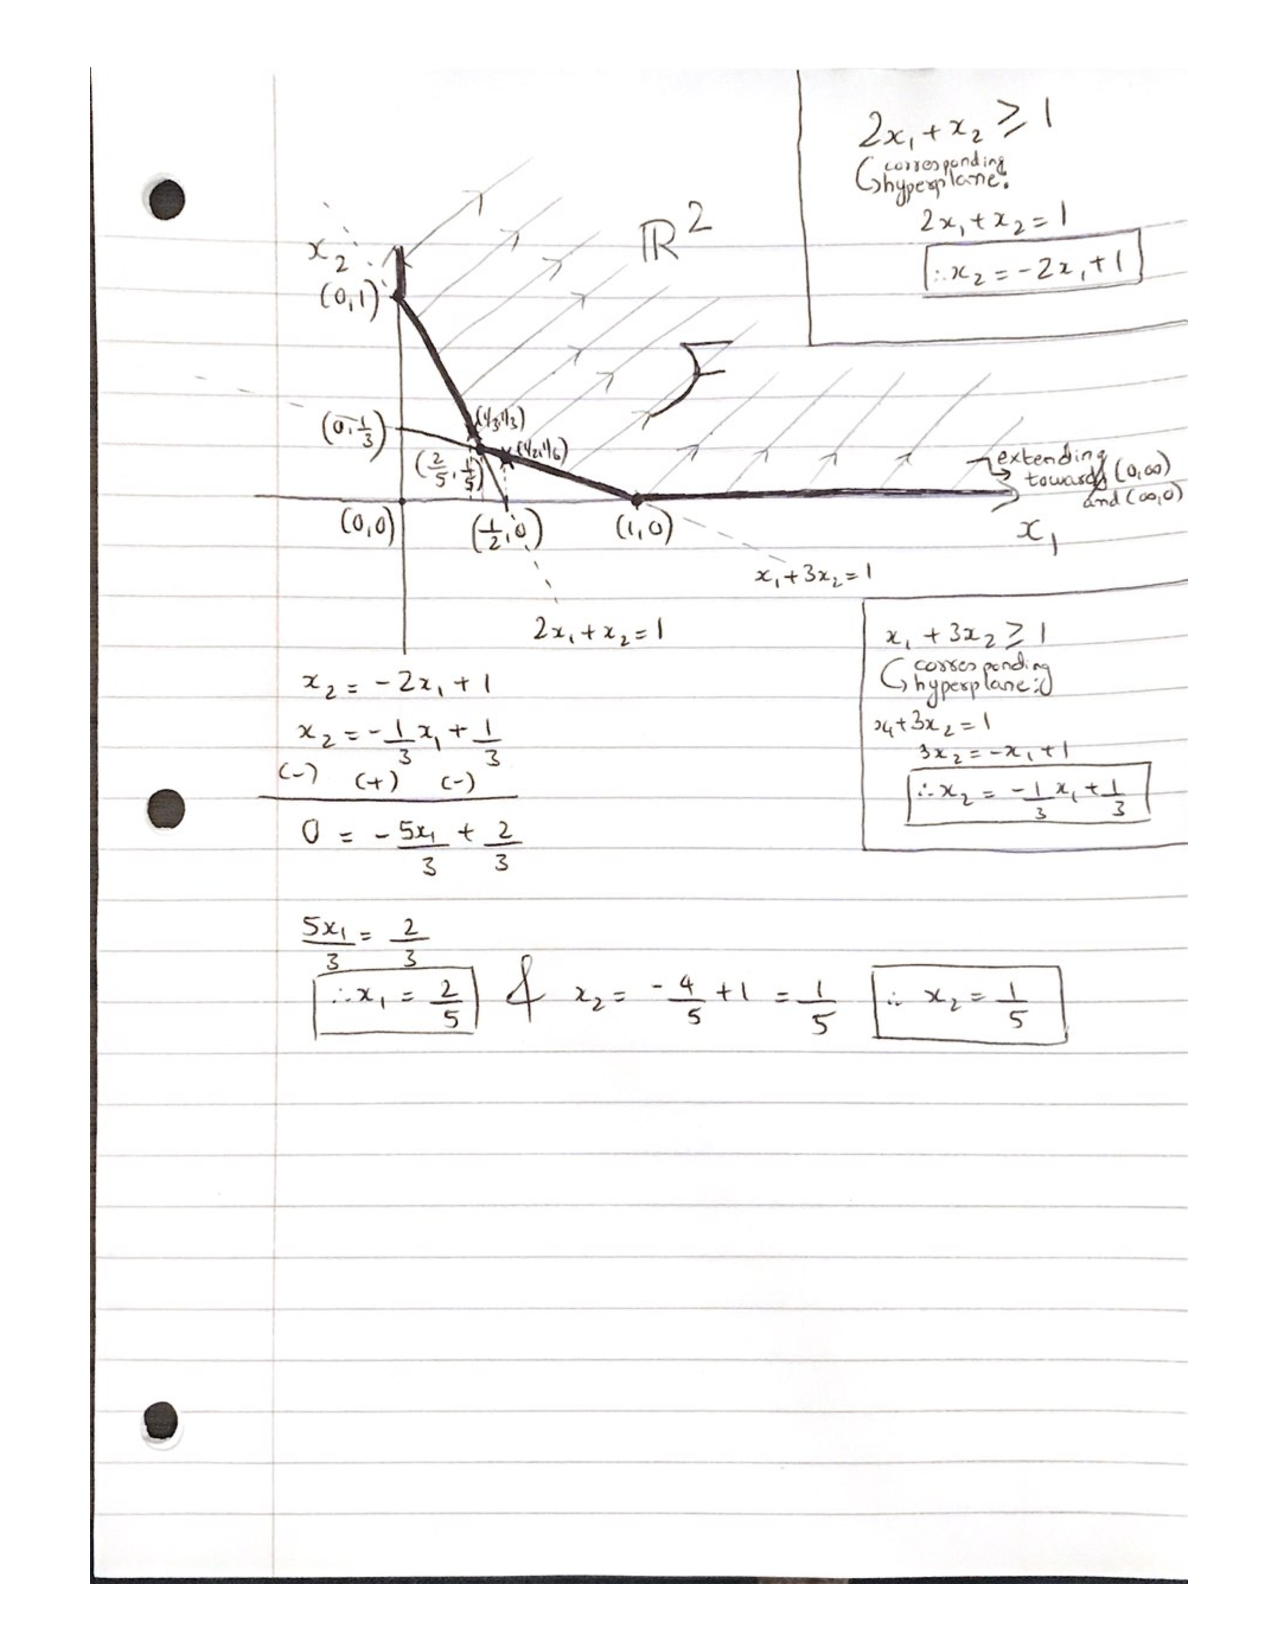
\includegraphics[width=0.8\textwidth,center]{Feasible_Set_Sketch.pdf}
    \caption{A sketch of the feasible set for the given problem - the feasible set for the given problem is convex hull of $(\infty,\ 0),\ (1,\ 0),\ (\frac{2}{5},\ \frac{1}{5}),\ (0,\ 1),\ and\ (0,\ \infty)$}
    \label{fig:1}
\end{figure}
\clearpage
\begin{enumerate}
    \item \[f_0(x_1,\ x_2)\ =\ x_1 + x_2\]
    The optimal point is,
    \\$x_1^*\ =\ \frac{2}{5}$
    \\$x_2^*\ =\ \frac{1}{5}$
    \\The optimum of this linear optimization problem is a corner point on the polyhedron.
    $f_0(x_1^*,\ x_2^*)\ =\ \frac{3}{5}$
    \item \[f_0(x_1,\ x_2)\ =\ -x_1 - x_2\]
    The optimal solution $f_0(x_1^*,\ x_2^*)$ goes to $-\infty$ as either $x_1 \rightarrow \infty$ or $x_2 \rightarrow \infty$.
    \\Therefore, this problem is \textbf{unbounded below}.
    \item \[f_0(x_1,\ x_2)\ =\ x_1\]
    The optimal set for this problem is the set of all points in $\mathbb{R}^2$ with $x_1 = 0$.
    \[X^*\ =\ \{x \in \mathcal{F}:\ x_1\ =\ 0\}\]
    where, $\mathcal{F}$ is the feasible set defined as follows,
    \[\mathcal{F}\ \equiv\ \{(x_1,\ x_2)\ \in\ \mathbb{R}^2:\ 2x_1 + x_2 \geq 1,\ x_1 + 3x_2 \geq 1,\ x_1 \geq 0,\ x_2 \geq 0\}\]
    $f_0(x_1^*,\ x_2^*)\ =\ 0$
    \item \[f_0(x_1,\ x_2)\ =\ \max\{x_1,\ x_2\}\]
    The optimal point is,
    \\$x_1^*\ =\ \frac{1}{3}$
    \\$x_2^*\ =\ \frac{1}{3}$
    \\$f(x_1^*,\ x_2^*)\ =\ \frac{1}{3}$
    \item \[f_0(x_1,\ x_2)\ =\ x_1^2 + 9x_2^2\]
    The optimal point is,
    \\$x_1^*\ =\ \frac{1}{2}$
    \\$x_2^*\ =\ \frac{1}{6}$
    \\$f(x_1^*,\ x_2^*)\ =\ \frac{1}{2}$
\end{enumerate}
\subsubsection{[Boyd] 4.3}
Quadratic Optimization Problem
\[\min\ \frac{1}{2} x^T P x + q^T x + r,\ s.t,\]
\[-1 \leq x_i \leq 1,\ i\ =\ 1,\ 2,\ 3\]
To prove that $x^*\ =\ (1,\ \frac{1}{2},\ -1)$ is the optimal point, we need to prove that,
\[\triangledown f_0(x^*)^T(y-x^*) \geq 0, \forall y \in \mathcal{F}\]
where,
\[\mathcal{F}\ \equiv\ \{x \in \mathbb{R}^3:\ -1 \leq x_i \leq 1\}\]
So,
\[\triangledown f_0(x)\ =\ \frac{2Px}{2} + q\]
\[\triangledown f_0(x)\ =\ Px + q\]
\[\triangledown f_0(x^*)\ =\ \begin{bmatrix}
21\\
14.5\\
-11\end{bmatrix} + \begin{bmatrix}
-22\\
-14.5\\
13\end{bmatrix}\]
\[\triangledown f_0(x^*)\ =\ \begin{bmatrix}
-1\\
0\\
2\end{bmatrix}\]
\[\triangledown f_0(x^*)^T(y-x^*)\ =\ \begin{bmatrix}
-1 & 0 & 2
\end{bmatrix}\begin{bmatrix}
y_1-1\\
y_2-\frac{1}{2}\\
y_3+1\end{bmatrix}\]
\[\triangledown f_0(x^*)^T(y-x^*)\ =\ -1(y_1 - 1) + 2(y_3 + 1)\]
For any $y \in \mathcal{F}$,
\[-1(y_1 - 1) + 2(y_3 + 1) \geq 0\]
which means that,
\[\triangledown f_0(x^*)^T(y-x^*) \geq 0,\ \forall y \in \mathcal{F}\]
Therefore, 
\[x^*\ =\ (1,\ \frac{1}{2},\ -1)\ is\ the\ optimal\ point\]
\setstcolor{red}
\end{document}